\chapter{Le projet}
\section{Présentation}
        \paragraph{}
        Open Orchestra est un CMS (Content Management  System) open source en développement depuis un peu plus d'un an. Il est actuellement en version bêta, la sortie de la première version est prévus pour le mois de septembre.
        \paragraph{}
        Il est basé sur le framework PHP MVC Symfony 2 et MongoDB. Open Orchestra offre bien-sûr les fonctionnalités attendues par tous CMS : gestion de contenu, médiathèque, contribution de page, gestion de version, utilisateurs, worklow, rôles,  multi-site, multi- langue,  multi-device , etc.
        \paragraph{}
        La grande particularité d'Open Orchestra est son faible couplage au niveau du code, mais aussi au niveau des solutions techniques, c'est-à-dire que l'on peut facilement remplacer ou étendre un de ses composants. Je reviendrais plus en détail sur ce point dans une section ultérieure.
        
        \section{Architecture}
       Avec Open Orchestra le \og Back-office \fg{} et le \og Front office \fg{} peuvent être dissociés dans deux applications Symfony différente. 

        Ce découpage a deux nombreux avantages, tous d'abord un seul \og Back-office \fg{}  peux gérer plusieurs sites (\og Front-office \fg{}), de plus cela permet de mettre \og Back-office \fg{} et le \og Front-office \fg{} sur des serveurs différents, l'unique condition est qu'ils doivent tous utiliser la même base de données.
        \paragraph{}
		Pour finir, Open Orchestra utilise une API RESTFull\footnote{REST (Representational State Transfer) est un style d'architecture qui définie différentes réglés (ressource identifié unitairement, utilisation des verbes HTTP POST, DELETE, PUT, GET) pour accéder et manipuler des ressources } pour  accéder, gérer ces différentes entités (pages, utilisateurs, contenus, etc).
	    \paragraph{}	
		Le schéma~\ref{architecture} présente l'architecture d'Open Orchestra avec un \og Back-office \fg{} qui gère plusieurs \og Fronts \fg{}.
		\begin{figure}[H]
        \begin{center}
          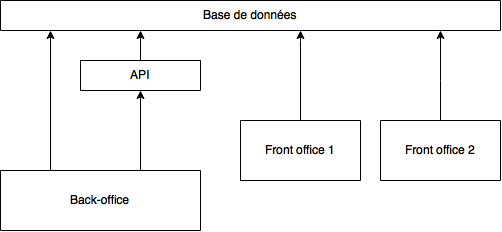
\includegraphics[scale=0.75]{images/architecture_open_orchestra}
        \end{center}
        \caption{Exemple d'architecture d'utilisation d'Open Orchestra}
        \label{architecture}
      \end{figure}

   
\chapter{Fonctionnalités}
	    \paragraph{}
	    Dans ce chapitre je vais vous présenter les différentes fonctionnalités d'Open Orchestra. Bien sûr, je ne vais pas tous les détailler, mais uniquement les points clés qui permettent une bonne compréhension du projet.
	      \section{Blocs}
	        \label{Blocs}  
	       \paragraph{}
	      Dans Open Orchestra tous les éléments visibles en front sont représentés par des blocs. Un bloc est simplement une entité avec des attributs qui varient selon le type de bloc. Chaque type de bloc sont indépendant, c'est-à-dire que eux seul connaissent leurs attributs, leurs façon de s'afficher en front ou en back-office ou encore la façon dont ils peuvent être contribué en back-office. 
	       \paragraph{}
	       Pour permettre cette indépendance, Open Orchestra utilise le design pattern stratégie. Le pattern stratégie permet de rendre une famille d'algorithmes interchangeables et ainsi  la possibilité d'exécuter un traitement spécifique selon le contexte.

          \paragraph{}
	       Comme le présente le diagramme de classe~\ref{pattern strategy} chaque bloc possède une classe qui indique comment il doit s'afficher pour cela la classe a deux méthodes, la première qui indique le bloc qu'elle supporte (\verb?support?) et la méthode \verb?show? qui fourni le rendu, d'un autre coté il y a une classe que appelé \verb?manager?  qui est la seule a connaitre toutes les stratégies des différents blocs. 
		\begin{figure}[H]
        \begin{center}
          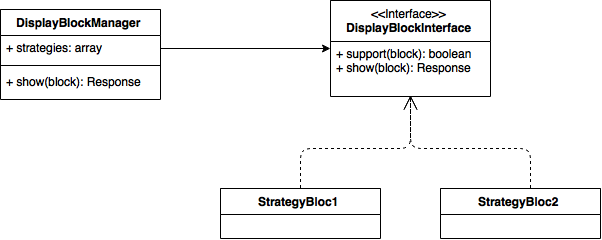
\includegraphics[scale=0.75]{images/strategy_block}
        \end{center}
        \caption{Utilisation du pattern stratégie pour l'affichage des bloc en front}
        \label{pattern strategy}
      \end{figure}
         \paragraph{}
	       Ainsi, lorsque que l'on désire afficher un bloc, il suffit de demander au manager d'afficher ce bloc, ce dernier va chercher parmi les stratégies qu'il connait laquelle supporte (méthode \verb?support?) le bloc et s'il en trouve une alors il exécute la méthode (\verb?show?) de la stratégie.
	        
	      	\paragraph{}
	      	Par défaut, le CMS propose de nombreux types blocs  comme par exemple un bloc pour lister un type de contenu, afficher un texte formaté, afficher un carrousel ou un média, un menu, une carte, un bloc de contact, etc.
	      \paragraph{}
	      	 Bien-sûr, il possible pour un intégrateur \footnote{Dans le cadre de ce rapport un intégrateur indique une personne ou une équipe qui utilise Open Orchestra afin de  l'étendre pour des besoins particuliers}, de créer son propre type de bloc, il lui suffit de développer les différentes stratégies (affichage en front et back-office, formulaire en back-office, etc) nécessaire à un bloc.  
         \section{Nodes}
         \paragraph{}
         Un des points central d'un CMS est les pages. Sur Open Orchestra les pages sont identifiées comme des noeuds (\og nodes \fg{}).
          Les nodes sont simplement des conteneurs qui contiennent des zones. Les zones permettent d'organiser la page, elles contiennent des sous-zones ou des blocs ce qui permet un découpage fin de la page pour simplifier sont organisation. 
         \paragraph{}
         Il existe trois types de nodes : 
         \begin{itemize}
         \item[]
         \item  Les nodes qui représentent les pages visibles en \og front \fg{}.
          \item[]
         \item  Les \og node tranverse \fg{} qui contiennent les blocs transverses, c'est-à-dire les blocs qui sont communs à plusieurs pages comme le bloc \og menu \fg{} ou encore le bloc \og footer \fg{}.
          \item[]
         \item Le dernier type de nodes sont ceux qui permettent de contribuer les pages d'erreurs (404, 503) d'un site.
         \end{itemize}
         \paragraph{}
		Le schéma~\ref{node} montre un exemple typique de page avec trois zones, le header qui contient un bloc menu, le footer un bloc footer et une zone principale découpé elle-même en deux zones avec un bloc de contact pour la zone de droite et un bloc de texte à gauche.
		\begin{figure}[H]
        \begin{center}
          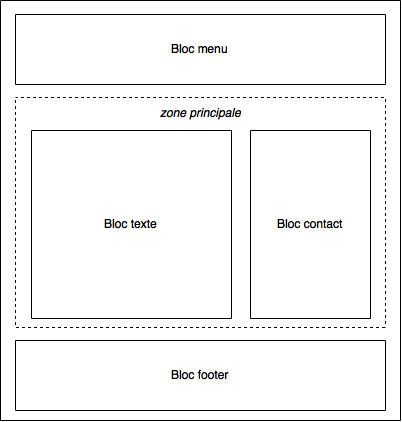
\includegraphics[scale=0.75]{images/node}
        \end{center}
        \caption{Exemple de page}
        \label{node}
      \end{figure}
         \section{Content type}
         Le second point important d'un CMS est les contenus avec Open Orchestra il est facile de créer des types de contenus (actualité, client, etc, ...).
          \paragraph{}
          En effet, Open Orchestra propose une approche graphique grâce à un formulaire pour créer ou éditer des types de contenus comme l'illustre la figure.
          Un type de contenu est composé de différent champs avec différente option, par exemple pour un champ de type texte il peut y avoir une option pour limiter le nombre de caractère ou encore une valeur par défaut.
          \paragraph{}
          Par défaut, Open Orchestra offre une liste de types de champs (date, texte, monnaie, média, email, entier, zone de texte riche, etc) qui comme pour tous les composants d'Open Orchestra peut être étendu par d'autre type de champ personnalisé. 
\chapter{Caractéristiques}
   \section{Performance}
   Open Orchestra a été développé pour supporter une charge de trafic importante. Pour cela le CMS exploite au niveau du front l'ESI (Edge Side Includes) couplé à un reverse proxy\footnote{Un reverse proxy est un serveur qui traite les requêtes en amont du serveur web. L'intérêt d'un reverse proxy est multiple gestion de cache, chiffrement, répartition de charge}.
   \paragraph{}
   L'ESI est un langage de balisage HTML qui permet de diviser une page en différent éléments dont les rendus sont faits dans différentes requêtes par le serveur web. Ce qui permet d'avoir un cache HTTP sur les différents éléments et ainsi rafraichir seulement les éléments obsolètes de la page et non toute la page.
   \paragraph{}
   Comme nous l'avons vu dans la section~\ref{block} sur Open Orchestra les pages sont déjà découpées en différent blocs ainsi l'utilisation de l'ESI est adapté et permet une amélioration significative des performances.
   \paragraph{}
   Si nous reprenons l'exemple de notre page (schéma~\ref{node}), le schéma~\ref{esi} présente le processus effectué par le serveur dans le cas où les blocs \verb?header? et \verb?footer? sont déjà en cache lorsqu'un utilisateur demande la page.
   		\begin{figure}[H]
        \begin{center}
          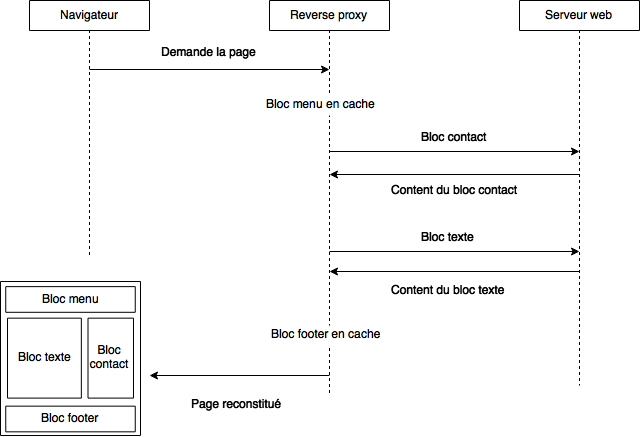
\includegraphics[scale=0.75]{images/esi}
        \end{center}
        \caption{Processus d'affichage d'une page qui utile l'ESI}
        \label{esi}
      \end{figure}
   
   \section{Modularités}
   Comme je vous l'expliquais en introduction la principale particularité d'Open Orchestra est sa modularité. Pour cela, les différents composants du CMS sont répartis dans différents bundles \footnote{Sous Symfony2 un bundle est un ensemble de fichiers structurés (contrôleur, entité commande, listener, formulaire) qui permettent d'implémenter une ou des fonctionnalités qui dans l'idéale peuvent être réutilisés dans différent projets}
   \paragraph{}
   \begin{itemize}
   \item \textbf{open-orchestra-base-bundle} : Classes communes au back-office et front-office
   \item \textbf{open-orchestra-base-api-bundle} : Api d'Open Orchestra
   \item \textbf{open-orchestra-base-api-mongo-model-bundle} : Implémentation des models nécessaires à l'api pour \verb?MongoDB? 
   \item \textbf{open-orchestra-cms-bundle} : Logique du back-office
   \item \textbf{open-orchestra-front-bundle} : Logique du front-office
   \item \textbf{open-orchestra-display-bundle} : Logique d'affichage des blocs en Front-office
   \item \textbf{open-orchestra-media-bundle} : Médiathèque d'Open Orchestra
   \item \textbf{open-orchestra-media-admin-bundle} : Administration de la médiathèque d'Open Orhcestra
   \item \textbf{open-orchestra-model-interface} : Interfaces des models utilisés par les autres bundles 
   \item \textbf{open-orchestra-model-bundle} : Implémentation des models pour \verb?MongoDB? 
   \item \textbf{open-orchestra-user-bundle} : Gestion des utilisateurs 
   \item \textbf{open-orchestra-workflow-function-bundle} : Système de workflow pour le back-office 
   \end{itemize}
   \paragraph{}
    Une application front-office n'a aucun intérêt à charger toute la logique du back-office ainsi grâce à ce découpage chaque application (front-office ou back-office) charge uniquement les composant qui lui est nécessaire.
   \paragraph{}
   De plus, cela permet de désactiver facilement une fonctionnalités. Par exemple, si un intégrateur n'a pas bessoin de gérer des médias il peut alors désactiver la médiathèque en n'utilisant pas les bundles (\verb?open-orchestra-media-bundle? et \verb?open-orchestra-media-admin-bundle?).

   \paragraph{}
   Un autre avantage est la facilité de remplacement d'un composants. Par défaut Open Orchestra utilise \verb?MongoDB? comme système de gestion de base de données, mais si un intégrateur veut utiliser un autre système comme \verb?Mysql? alors il lui suffit d'écrire son propre \newline  \verb?open-orchestra-model-bundle? qui utilise bien-sûr les différentes interfaces de  \newline  \verb?open-orchestra-model-interface? adapté a \verb?Mysql?.